一曰茶,二曰檟,三曰蔎,四曰茗,五曰荈

\begin{flushright}
------陆羽 《茶经》
\end{flushright}

茶(土耳其语:çay)流行于土耳其以及海外土耳其人中。土耳其茶文化同时影响了阿塞拜疆在内的巴尔干半岛诸国。土耳其的人均茶消耗量世界第一,达到2.5
kg/人/年,紧随其后的是英国(2.1 kg/人/年)。

香柠檬烯(bergamotene)及其衍生物\textbf{1}-\textbf{4}属倍半萜类化合物,皆为蒎烷类单萜的类似物。香柠檬烯存在于香柠檬油中,是格雷伯爵茶香和味的来源。

\begin{figure}[h]
	\centering
	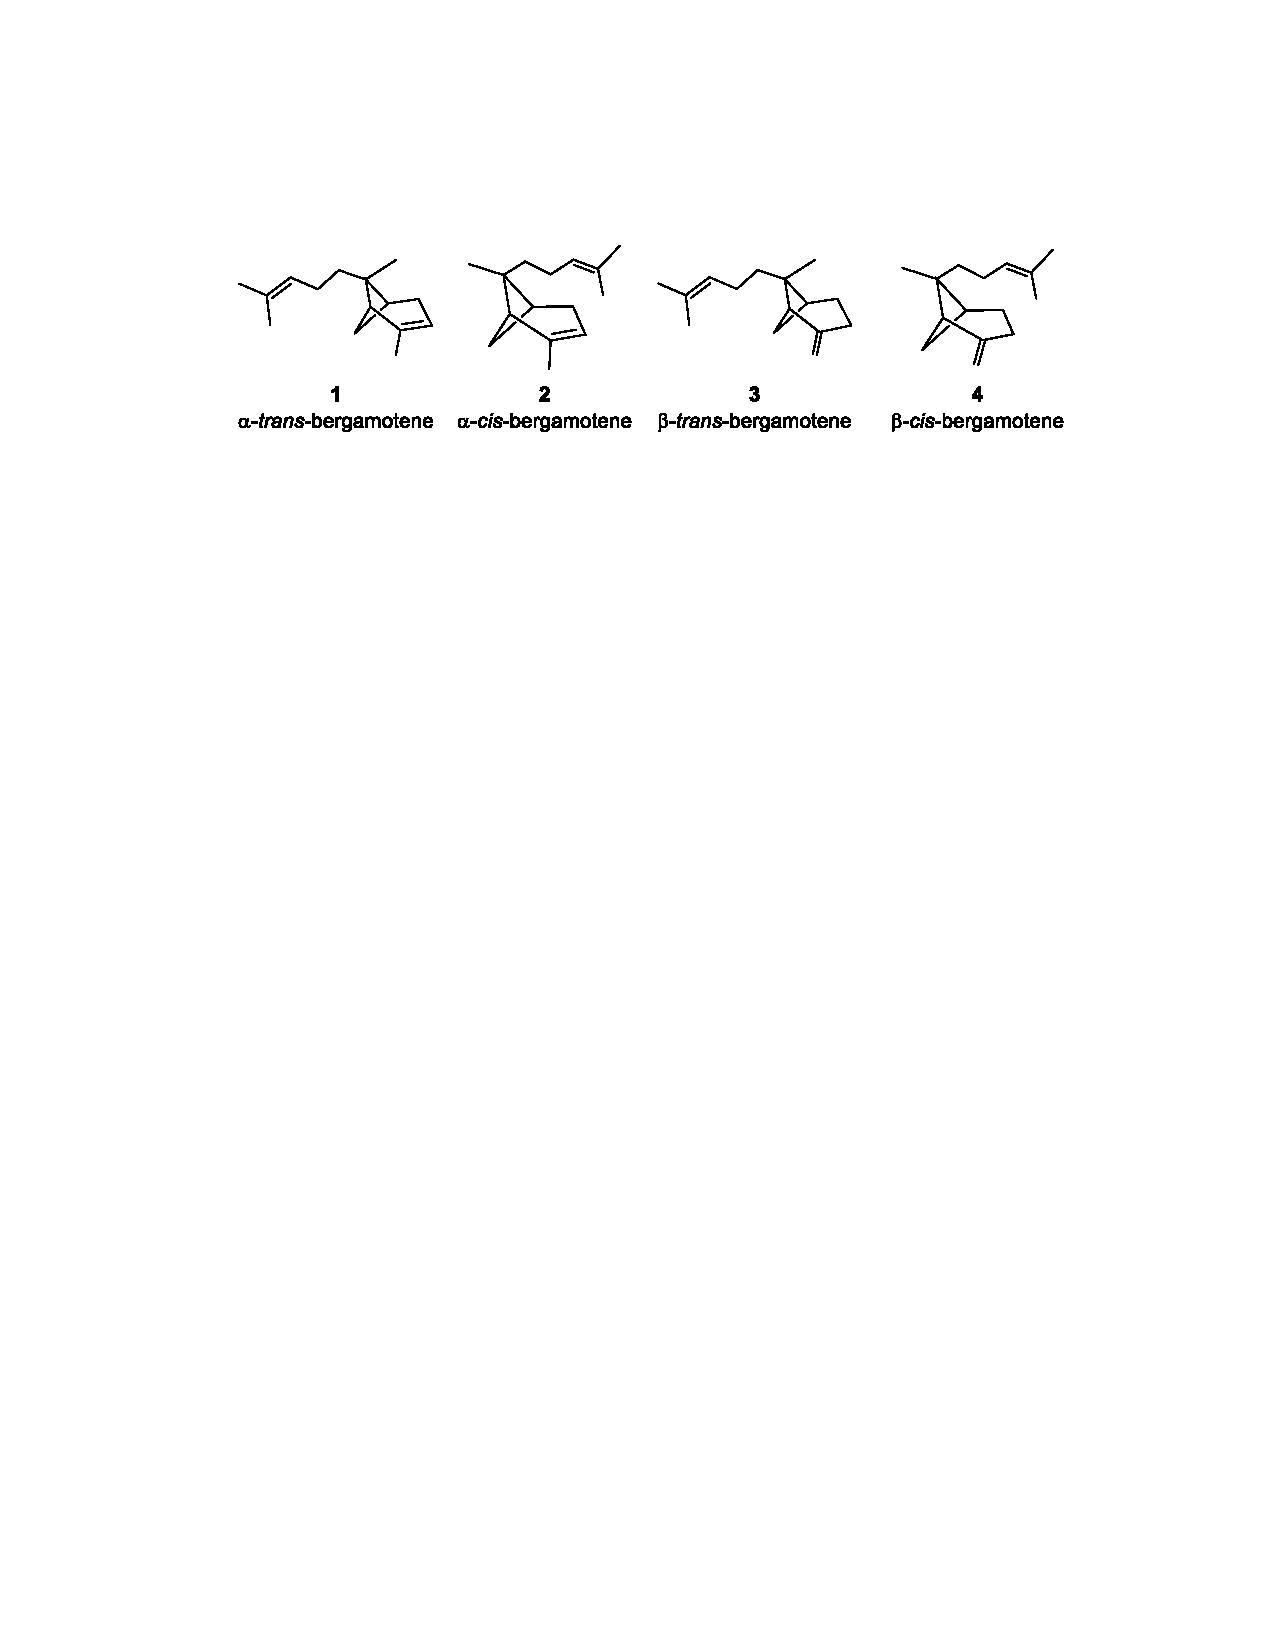
\includegraphics[width=13cm]{./pic/t3-1.pdf}
\end{figure}

\noindent\textbf{3.1.}以下的反应图示出了$\alpha$-反式香柠檬烯\textbf{1}的合成路线。画出产物\textbf{A}-\textbf{G}的结构。

\noindent\textbf{3.2.} 从\textbf{A}到\textbf{B}的转化中,试剂Me\textsubscript{3}NO的作用是什么?

\begin{figure}[h]
	\centering
	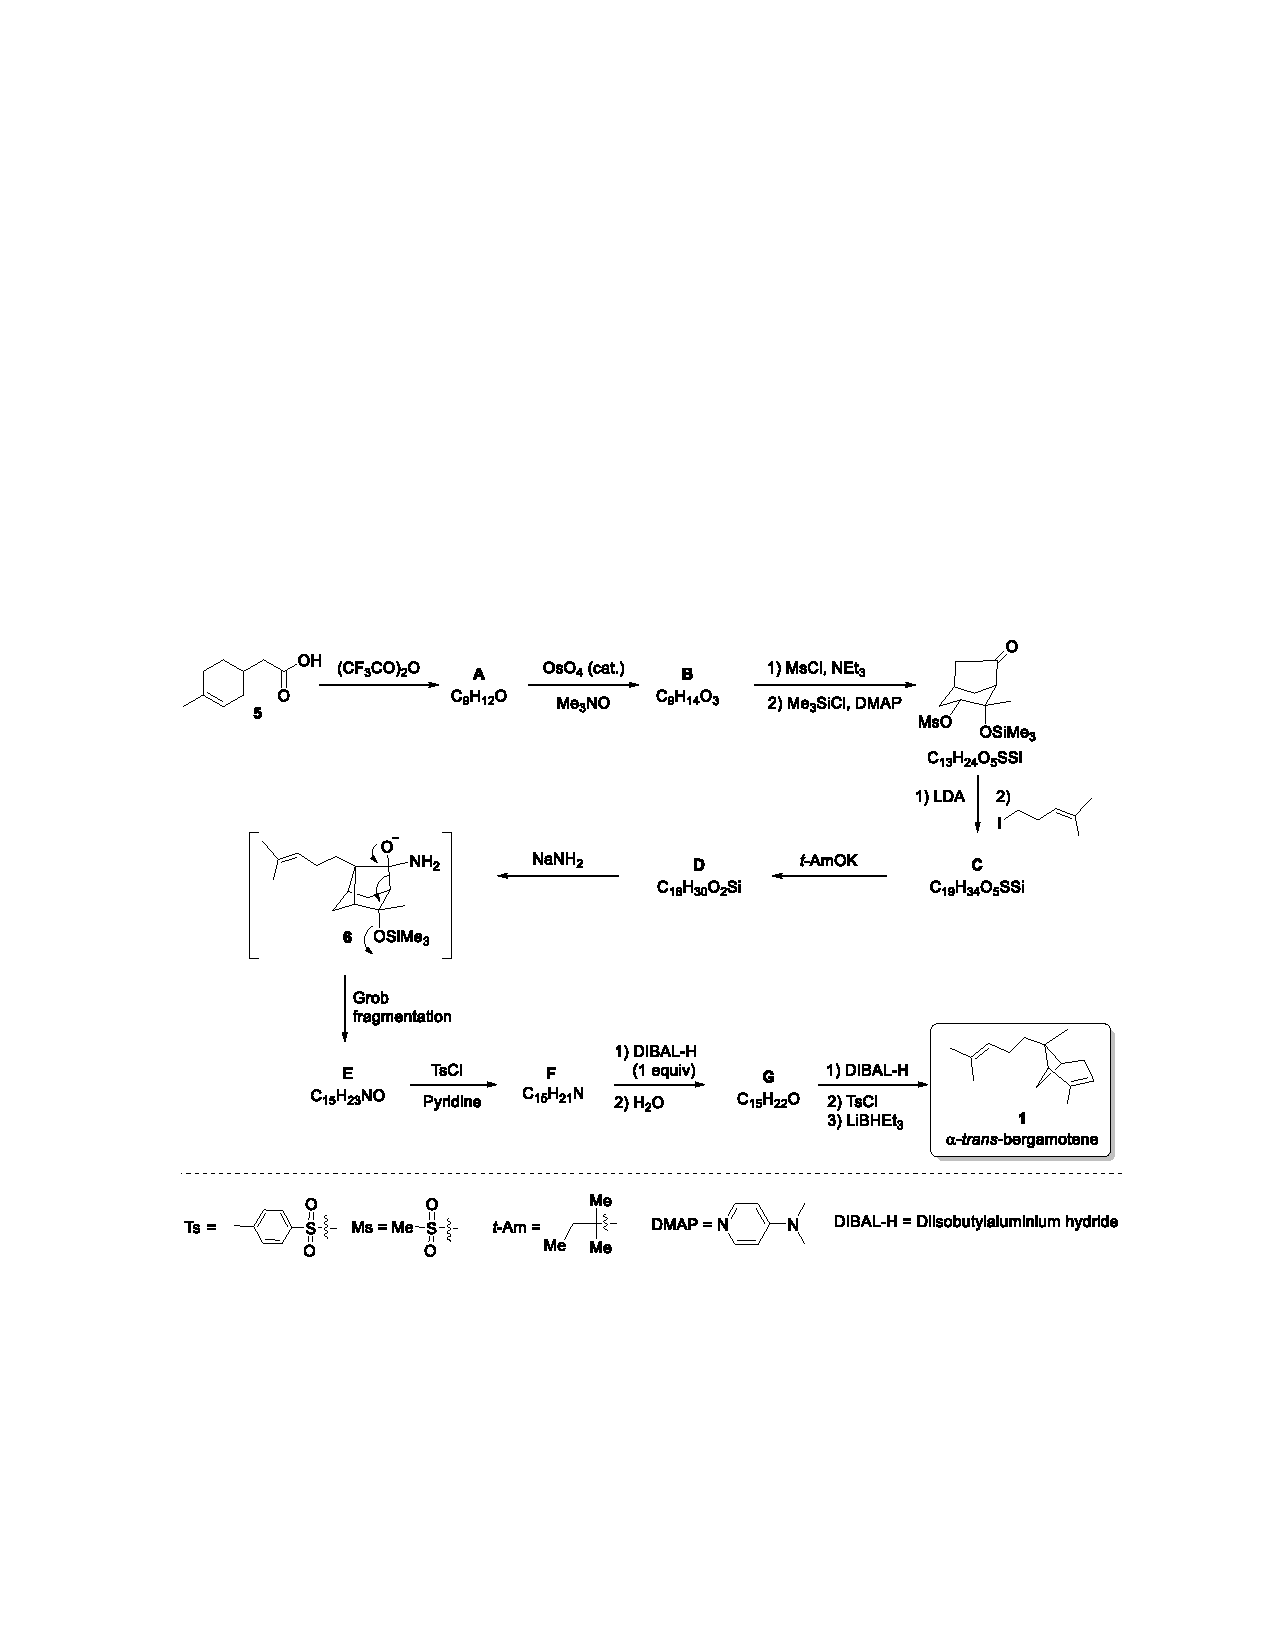
\includegraphics[width=16cm]{./pic/t3-2.pdf}
\end{figure}
